\documentclass[a4paper,10pt]{article}
\usepackage{fullpage}
\usepackage{float}
\usepackage[english]{babel}
\usepackage{graphicx,subfig,wrapfig}
\usepackage{amsmath,amsfonts,amsthm,amssymb}
\usepackage{fancyhdr,fancybox,color}
\usepackage{enumerate}
\usepackage{multirow}
\usepackage[amssymb]{SIunits}
\definecolor{MyBlue}{rgb}{0,0.3,0.6}

\usepackage{tcolorbox}
\definecolor{mgray}{gray}{0.85}
\definecolor{mpurple}{HTML}{68236D}
\usepackage[colorlinks=true,
linkcolor=MyBlue,
plainpages=false,
citecolor=MyBlue,
urlcolor=MyBlue]{hyperref}
\usepackage[all]{hypcap}
\usepackage[url=false,
backend=bibtex,
style=authoryear-comp,
doi=true,
isbn=true,
backref=false,
dashed=false,
maxcitenames=2,
maxbibnames=99,
natbib=true]{biblatex}
\DeclareNameAlias{author}{last-first}
\renewbibmacro{in:}{}
\addbibresource{../_logosAndRef/references.bib}
\nonfrenchspacing
\begin{document}
\noindent Chair: Physics of Fluids Department

\begin{center}
	\begin{LARGE}
	From Champagne to Coughs: Modelling Droplet Formation
	\end{LARGE}
\end{center}

\noindent Hold your palm over a glass of champagne (fig.~\ref{fig:champange}) and feel the mist of tiny droplets landing on your skin. These droplets, launched by bursting bubbles, carry everything from wine aromatics to -- in other contexts -- airborne pathogens.

\begin{figure}[H]
\begin{center}
	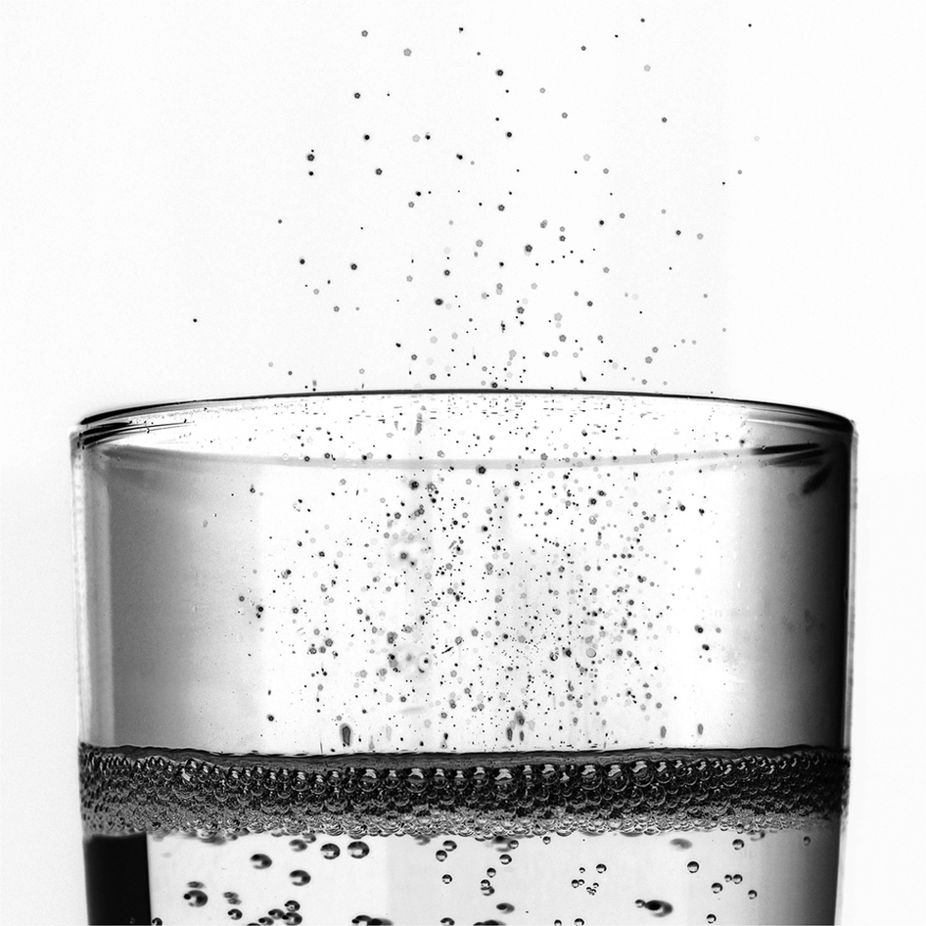
\includegraphics[width=0.4\textwidth]{champagne.jpg}
	\caption{\citet{ghabache2016evaporation} reported the collapse of numerous bubbles at the free surface, emitting a cloud of tiny droplets, which is characteristic of champagne and other sparkling wines and enhances the sensual experience of the taster.}
	\label{fig:champange}
\end{center}
\end{figure}

\begin{tcolorbox}[colback=mgray,colframe=mpurple,title=TL;DR]
	Investigate how bubbles burst in complex fluids that behave like both liquids and elastic solids -- from volcanic mudpots to respiratory mucus. Using computational fluid dynamics simulations with the open-source \href{https://comphy-lab.org/MultiRheoFlow}{Basilisk C} solver, you'll discover how viscosity and elasticity compete to control jet formation and droplet ejection when bubble cavities collapse. Your simulations will map regimes where elastic stresses suppress or enhance jetting. Working with international collaborators at Twente and Delft who provide experimental validation, you'll connect fundamental physics to applications including aerosol formation in sparkling beverages and respiratory droplet generation during coughing. The project combines multiphase flow physics, non-Newtonian fluid mechanics, and high-performance computing to address open questions in interfacial dynamics with direct relevance to disease transmission modelling.
\end{tcolorbox}

\section*{Description}

Bubble bursting at liquid surfaces creates spectacular jets that eject droplets into the air, a phenomenon ubiquitous from ocean spray to volcanic mudpots (see \href{https://www.youtube.com/watch?v=a9hUsVq9q7U}{YouTube link}) to respiratory disease transmission \citep{walls2017quantifying,bourouiba2021fluid,sanjay_lohse_jalaal_2021,balasubramanianBurstingBubbleElastoviscoplastic2024,dixit2024viscoelastic}. While the physics in simple Newtonian fluids is well-established \citep{duchemin2002jet, walls2015jet, deike2018dynamics, gordillo2019capillary}, we lack understanding of bubble bursting in complex non-Newtonian fluids -- particularly elastoviscoplastic materials that flow like water yet store elastic energy like rubber bands. 
This project investigates bubble collapse dynamics, jet formation, and droplet ejection in non-Newtonian fluids using cutting-edge computational fluid dynamics simulations. 
You'll systematically vary fluid properties to discover how viscosity and elasticity compete to control jet heights and droplet sizes, working in parallel with laboratory experiments for direct validation. Your findings will illuminate fundamental fluid physics while directly informing models of respiratory droplet formation during coughing and sneezing -- crucial for understanding airborne disease transmission.

	
\begin{figure}[H]
\begin{center}
	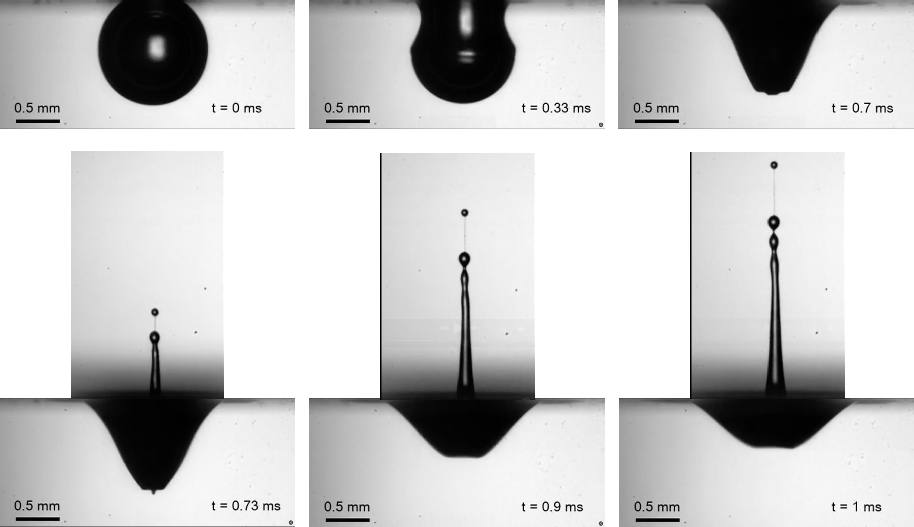
\includegraphics[width=0.9\textwidth]{schematic.pdf}
	\caption{Observation of the time evolution of the open bubble cavity. The lower rows display two views: the top view is above the water surface, while the bottom view is below the surface. }
	\label{Figure::Waves}
\end{center}
\end{figure}

\section*{Deep dive}

When a bubble bursts at a free surface, it creates an open cavity that collapses under surface tension forces. Capillary waves propagate along the cavity interface, focusing at the cavity bottom to generate an upward jet (Worthington jet) that subsequently breaks into droplets (see figs.~\ref{Figure::Waves}). The governing dynamics involve the interplay between inertia, surface tension, viscosity, and in viscoelastic fluids, elastic stresses and relaxation time of these elastic stresses.

\section*{What you will do and what you will learn?}

\begin{enumerate}
\item You will learn about the physics of fluids, and science underlying non-Newtonian fluid flows. 
\item You will learn how to utilize state-of-the-art computational tools to study real life physics. 
\item You will have access to a read-to-use codebase (available on \href{https://comphy-lab.org/MultiRheoFlow}{GitHub}).
\item As a part of the \href{https://comphy-lab.org}{CoMPhy lab}, you will learn and adapt open-source coding principles. 
\item You will learn how to collaborate with a diverse group of researchers, specifically with other numericists, experimentalists and theoreticians.

\end{enumerate}

If you have any questions, feel free to contact \href{mailto:a.k.dixit@utwente.nl}{Ayush} (details below).
\begin{center}
\begin{tabular}{|l|l|l|}
\hline \textbf{Supervision} & \textbf{E-mail} & \textbf{Office} \\
\hline Ayush Dixit M.Sc. & \href{mailto:a.k.dixit@utwente.nl}{a.k.dixit@utwente.nl} & Meander 250 \\
\hline Coen Verschuur & \href{mailto:c.i.verschuur@utwente.nl}{c.i.verschuur@utwente.nl} & Meander 114B \\
\hline \multirow{2}{*}{Dr. Vatsal Sanjay} & \href{mailto:vatsal.sanjay@comphy-lab.org}{vatsal.sanjay@comphy-lab.org} & \multirow{2}{*}{Durham University} \\
& \href{mailto:vatsal.sanjay@durham.ac.uk}{vatsal.sanjay@durham.ac.uk} & \\
\hline Dr. Alexandros Oratis   & \href{mailto:a.t.oratis@tudelft.nl}{a.t.oratis@tudelft.nl}& TU Delft \\
\hline Prof. Dr. Detlef Lohse F.R.S. & \href{mailto:d.lohse@utwente.nl}{d.lohse@utwente.nl} & Meander 261  \\
\hline
\end{tabular}
\end{center}
\printbibliography
\end{document}
